% move all configuration stuff into one file so we can focus on the content
\documentclass[hyperref={pdfpagelabels=false,colorlinks=true,linkcolor=white,urlcolor=blue}]{beamer}

%%%%%%%%%%%%%%%%%%%%%%%%%%%%%%%%%%%%%%%%%%%%%%%%%%%%%%%%%%%%%%%%%%%%%%%%%%%%%%%%%%
%%%%%%%%%%%%%%%%%%%%%%%%%%%%%%%%%%%%%%%%%%%%%%%%%%%%%%%%%%%%%%%%%%%%%%%%%%%%%%%%%%
% packages
\usepackage{pict2e}
\usepackage{epic}
\usepackage{amsmath,amsfonts,amssymb}
\usepackage{units}
\usepackage{fancybox}
\usepackage[absolute,overlay]{textpos} 
\usepackage{media9} % avi2flv: "C:\Program Files\ffmpeg\bin\ffmpeg.exe" -i TuneFreqFilterbank.avi -b 600k -s 441x324 -r 15 -acodec copy TuneFreqFilterbank.flv
\usepackage{silence}
\usepackage[backend=bibtex,style=ieee]{biblatex}
\WarningFilter{biblatex}{Patching footnotes failed}
\AtEveryCitekey{\iffootnote{\tiny}{}}
\addbibresource{references}

%%%%%%%%%%%%%%%%%%%%%%%%%%%%%%%%%%%%%%%%%%%%%%%%%%%%%%%%%%%%%%%%%%%%%%%%%%%%%%%%%%
%%%%%%%%%%%%%%%%%%%%%%%%%%%%%%%%%%%%%%%%%%%%%%%%%%%%%%%%%%%%%%%%%%%%%%%%%%%%%%%%%%
% relative paths
\graphicspath{{graph/}}

%%%%%%%%%%%%%%%%%%%%%%%%%%%%%%%%%%%%%%%%%%%%%%%%%%%%%%%%%%%%%%%%%%%%%%%%%%%%%%%%%%
%%%%%%%%%%%%%%%%%%%%%%%%%%%%%%%%%%%%%%%%%%%%%%%%%%%%%%%%%%%%%%%%%%%%%%%%%%%%%%%%%%
% colors
\definecolor{gtgold}{HTML}{E0AA0F} %{rgb}{0.88,0.66,1,0.06} [234, 170, 0]/256

%%%%%%%%%%%%%%%%%%%%%%%%%%%%%%%%%%%%%%%%%%%%%%%%%%%%%%%%%%%%%%%%%%%%%%%%%%%%%%%%%%
%%%%%%%%%%%%%%%%%%%%%%%%%%%%%%%%%%%%%%%%%%%%%%%%%%%%%%%%%%%%%%%%%%%%%%%%%%%%%%%%%%
% math
\DeclareMathOperator*{\argmax}{argmax}
\DeclareMathOperator*{\argmin}{argmin}
\DeclareMathOperator*{\atan}{atan}
\DeclareMathOperator*{\arcsinh}{arcsinh}
\DeclareMathOperator*{\sign}{sign}
\DeclareMathOperator*{\tcdf}{tcdf}
\DeclareMathOperator*{\si}{sinc}
\DeclareMathOperator*{\princarg}{princarg}
\DeclareMathOperator*{\arccosh}{arccosh}
\DeclareMathOperator*{\hwr}{HWR}
\DeclareMathOperator*{\flip}{flip}
\DeclareMathOperator*{\sinc}{sinc}
\newcommand{\e}{{e}}
\newcommand{\jom}{\mathrm{j}\omega}
\newcommand{\jOm}{\mathrm{j}\Omega}
\newcommand   {\mat}[1]    		{\boldsymbol{\uppercase{#1}}}		%bold
\renewcommand {\vec}[1]    		{\boldsymbol{\lowercase{#1}}}		%bold

%%%%%%%%%%%%%%%%%%%%%%%%%%%%%%%%%%%%%%%%%%%%%%%%%%%%%%%%%%%%%%%%%%%%%%%%%%%%%%%%%%
%%%%%%%%%%%%%%%%%%%%%%%%%%%%%%%%%%%%%%%%%%%%%%%%%%%%%%%%%%%%%%%%%%%%%%%%%%%%%%%%%%
% media9
\newcommand{\includeaudio}[1]{{\includemedia[
                        addresource=audio/#1.mp3,
                        width=5mm,
                        height=5mm,
                        activate=onclick,
                        flashvars={
                            source=audio/#1.mp3  
                            &autoPlay=true
                        }]
                        {\includegraphics[width=5mm, height=5mm]{SpeakerIcon}}
                        {APlayer.swf}}}
\newcommand{\audioautoplay}[1]{{\begin{center}\includemedia[
                            addresource=audio/#1.mp3,
                            width=.1\linewidth,
                            height=.01\linewidth,
                            activate=pageopen,
                            flashvars={
                                source=audio/#1.mp3  
                                &autoPlay=true
                            }]
                            {}
                            {APlayer.swf}\end{center}}}

\newcommand{\includevideo}[1]{{\begin{center}\includemedia[
                        addresource=video/#1.mp4,
                        width=0.8\linewidth,
                        height=0.4\linewidth,
                        activate=onclick,
                        flashvars={
                            source=video/#1.mp4  
                            &autoPlay=true
                        }]
                        {}
                        {VPlayer.swf}\end{center}}}
\newcommand{\videowithmatlab}[1]{{\begin{center}\includemedia[
                        addresource=video/animate#1.mp4,
                        width=0.8\linewidth,
                        height=0.4\linewidth,
                        activate=onclick,
                        flashvars={
                            source=video/animate#1.mp4  
                            &autoPlay=true
                        }]
                        {}
                        {VPlayer.swf}\end{center}\addreference{matlab source: matlab/animate#1.m}}}
                        

%%%%%%%%%%%%%%%%%%%%%%%%%%%%%%%%%%%%%%%%%%%%%%%%%%%%%%%%%%%%%%%%%%%%%%%%%%%%%%%%%%
%%%%%%%%%%%%%%%%%%%%%%%%%%%%%%%%%%%%%%%%%%%%%%%%%%%%%%%%%%%%%%%%%%%%%%%%%%%%%%%%%%
% other commands
\newcommand{\question}[1]{\vspace{-4mm}
                          \setbeamercovered{invisible}
                          \begin{columns}
                            \column{.7\textwidth}
                                \textbf{#1}\\
                            \column{.3\textwidth}
                                \begin{flushright}
                                     \includegraphics[scale=.5]{question_mark}
                                \end{flushright}
                                \vspace{6mm}
                          \end{columns}\pause\vspace{-6mm}}

\newcommand{\toremember}[1]{\vspace{-4mm}
                          \begin{columns}
                            \column{.7\textwidth}
                                \textbf{#1}\\
                            \column{.3\textwidth}
                                \begin{flushright}
                                     \includegraphics[scale=.5]{exclamation_mark}
                                \end{flushright}
                                \vspace{6mm}
                          \end{columns}\vspace{-6mm}}

\newcommand{\matlabexercise}[1]{\vspace{-4mm}
                          \setbeamercovered{invisible}
                          \begin{columns}
                            \column{.7\textwidth}
                                \textbf{matlab exercise}: #1
                            \column{.3\textwidth}
                                \begin{flushright}
                                     \includegraphics[scale=.5]{logo_matlab}
                                \end{flushright}
                                \vspace{6mm}
                          \end{columns}}

\newcommand{\addreference}[1]{                    
                    \begin{textblock*}{\baselineskip }(1.15\textwidth,.5\textheight)
                        \rotatebox{90}{\tiny #1}
                    \end{textblock*}}
                    
\newcommand{\figwithmatlab}[1]{
                    \begin{figure}
                        \centering
                        \includegraphics{#1}
                        \label{fig:#1}
                    \end{figure}
                    
                    \addreference{matlab source: matlab/display#1.m}}                    
\newcommand{\figwithref}[2]{
                    \begin{figure}
                        \centering
                        \includegraphics{#1}
                        \label{fig:#1}
                    \end{figure}
                    
                    \addreference{#2}}                    

%%%%%%%%%%%%%%%%%%%%%%%%%%%%%%%%%%%%%%%%%%%%%%%%%%%%%%%%%%%%%%%%%%%%%%%%%%%%%%%%%%
%%%%%%%%%%%%%%%%%%%%%%%%%%%%%%%%%%%%%%%%%%%%%%%%%%%%%%%%%%%%%%%%%%%%%%%%%%%%%%%%%%
% units
\setlength{\unitlength}{1mm}

%%%%%%%%%%%%%%%%%%%%%%%%%%%%%%%%%%%%%%%%%%%%%%%%%%%%%%%%%%%%%%%%%%%%%%%%%%%%%%%%%%
%%%%%%%%%%%%%%%%%%%%%%%%%%%%%%%%%%%%%%%%%%%%%%%%%%%%%%%%%%%%%%%%%%%%%%%%%%%%%%%%%%
% counters
\newcounter{i}
\newcounter{iXOffset}
\newcounter{iYOffset}
\newcounter{iXBlockSize}
\newcounter{iYBlockSize}
\newcounter{iYBlockSizeDiv2}
\newcounter{iDistance}


%%%%%%%%%%%%%%%%%%%%%%%%%%%%%%%%%%%%%%%%%%%%%%%%%%%%%%%%%%%%%%%%%%%%%%%%%%%%%%%%%%
%%%%%%%%%%%%%%%%%%%%%%%%%%%%%%%%%%%%%%%%%%%%%%%%%%%%%%%%%%%%%%%%%%%%%%%%%%%%%%%%%%
% theme & layout
\usetheme{Frankfurt}
\beamertemplatenavigationsymbolsempty
%\setbeamertemplate{frametitle}[smoothbars theme]
\setbeamertemplate{frametitle}
{
    \begin{beamercolorbox}[ht=1.8em,wd=\paperwidth]{frametitle}
        \vspace{-.1em}%
        \hspace{.2em}{\strut\insertframetitle\strut}
        
        \hspace{.2em}\small\strut\insertframesubtitle\strut
        %\hfill
        %\includegraphics[height=.8cm,keepaspectratio]{CenterMusicTechnology-solid-2lines-white-CoAtag}
        
    \end{beamercolorbox}
    \begin{textblock*}{100mm}(8.3cm,.65cm)
        \includegraphics[height=.8cm,keepaspectratio]{CenterMusicTechnology-solid-2lines-white-CoAtag}
    \end{textblock*}
}

% set this to ensure bulletpoints without subsections
\usepackage{remreset}
\makeatletter
\@removefromreset{subsection}{section}
\makeatother
\setcounter{subsection}{1}

%---------------------------------------------------------------------------------
% appearance
\setbeamercolor{structure}{fg=gtgold}
\setbeamercovered{transparent} %invisible
\setbeamercolor{bibliography entry author}{fg=black}
\setbeamercolor*{bibliography entry title}{fg=black}
\setbeamercolor*{bibliography entry note}{fg=black}
%---------------------------------------------------------------------------------
% fontsize
\let\Tiny=\tiny

%%%%%%%%%%%%%%%%%%%%%%%%%%%%%%%%%%%%%%%%%%%%%%%%%%%%%%%%%%%%%%%%%%%%%%%%%%%%%%%%%%
%%%%%%%%%%%%%%%%%%%%%%%%%%%%%%%%%%%%%%%%%%%%%%%%%%%%%%%%%%%%%%%%%%%%%%%%%%%%%%%%%%
% warnings
\pdfsuppresswarningpagegroup=1

%%%%%%%%%%%%%%%%%%%%%%%%%%%%%%%%%%%%%%%%%%%%%%%%%%%%%%%%%%%%%%%%%%%%%%%%%%%%%%%%%%
%%%%%%%%%%%%%%%%%%%%%%%%%%%%%%%%%%%%%%%%%%%%%%%%%%%%%%%%%%%%%%%%%%%%%%%%%%%%%%%%%%
% title information
\title[]{MUSI-6201~---~Computational Music Analysis}   
\author[alexander lerch]{alexander lerch} 
%\institute{~}
%\date[Alexander Lerch]{}
\titlegraphic{\vspace{-16mm}\includegraphics[scale=.25]{title}}


\subtitle{Part 6.2: Frequency Resolution of Pitch Tracking Solutions}

%%%%%%%%%%%%%%%%%%%%%%%%%%%%%%%%%%%%%%%%%%%%%%%%%%%%%%%%%%%%%%%%%%%%%%%%%%%%
\begin{document}
    % generate title page
	

\begin{frame}
    \titlepage
    %\vspace{-5mm}
    \begin{flushright}
        \href{http://www.gtcmt.gatech.edu}{\includegraphics[height=.8cm,keepaspectratio]{logo_GTCMT_black}}
    \end{flushright}
\end{frame}


    \section[overview]{lecture overview}
        \begin{frame}{instantaneous features}{overview}
            \begin{itemize}
                \item   \textbf{text book}  
                    \begin{itemize}
                        \item   \href{http://ieeexplore.ieee.org/xpl/articleDetails.jsp?tp=&arnumber=6331119&}{\underline{\textit{Chapter 2: Fundamentals} (pp.~21--23)}}
                        \item   \href{http://ieeexplore.ieee.org/xpl/articleDetails.jsp?tp=&arnumber=6331122&}{\underline{\textit{Chapter 5: Tonal Analysis} (pp.~91--93)}}
                    \end{itemize}
                \bigskip
                \item<2->   \textbf{lecture content}
                    \begin{itemize}
                        \item<2->   frequency resolution of pitch tracking
                            \begin{itemize}
                                \item   time domain vs.\ frequency domain resolution
                                \item   possible workarounds
                            \end{itemize}
                    \end{itemize}
            \end{itemize}
        \end{frame}

    \section[intro]{introduction}
        \begin{frame}{pitch detection resolution}{introduction}
            \begin{itemize}
                \item fundamental frequency detection on digital signals
                \item[$\Rightarrow$] quantized result/frequency resolution
            \end{itemize}
            
            \question{what is the maximum error the algorithms make}
            
            \begin{itemize}
                \item   \textbf{time domain}:
                    \begin{itemize}
                        \item   detection of period length
                        \item[$\Rightarrow$] maximum error is distance between two samples
                    \end{itemize}
                \item<3->   \textbf{frequency domain}:
                    \begin{itemize}
                        \item detection of frequency bin
                        \item[$\Rightarrow$] maximum error is distance between two frequency bins
                    \end{itemize}
                \bigskip
                \item<4->[] \textbf{BUT}
                    \begin{itemize}
                        \item<5->   a more meaningful error metric is neither \unit{s} nor \unit{Hz} but \textit{Cent}
                    \end{itemize}
            \end{itemize}
        \end{frame}
        \begin{frame}{pitch detection resolution}{time domain (e.g., ACF)}
            period length quantized to multiple of inter-sample interval 
            \begin{equation}
                T_\mathrm{Q} = j\cdot T_{\mathrm{S}}
            \end{equation}
            \figwithmatlab{TimeDomainPitchError}
        \end{frame}
        \begin{frame}{pitch detection resolution}{frequency domain (e.g., HPS)}
		frequency quantized to multiple of inter-bin interval
		 \begin{equation}
		 	f_\mathrm{Q} = k\cdot\frac{f_{\mathrm{S}}}{\mathcal{K}} 
		 \end{equation}
		 \only<2>
		 {
			\begin{footnotesize}\begin{table}
				\centering
				\begin{tabular}{lccc} %{c|p{12mm}p{12mm}p{12mm}p{12mm}p{12mm}p{12mm}p{12mm}}
                    \\ \hline
                    \bf{\emph{$\mathcal{K}$}}	 & \bf{\emph{$\Delta f\;[\unit{Hz}]$}}	 & \bf{\emph{$k_\mathrm{ST}$}}	 & \bf{\emph{$f(k_\mathrm{ST})\;[\unit{Hz}]$}}\\ 
                     \hline
                    \bf{256}	 & 187.5	 & 35	 & 6562.5\\
                    \bf{512}	 & 93.75	 & 35	 & 3281.25\\
                    \bf{1024}	 & 46.875	 & 35	 & 1640.625\\
                    \bf{2048}	 & 23.4375	 & 35	 & 820.3125\\
                    \bf{4096}	 & 11.7188	 & 35	 & 410.1563\\
                    \bf{8192}	 & 5.8594	 & 35	 & 205.0781\\
                    \bf{16384}	 & 2.9297	 & 35	 & 102.5391\\
				\end{tabular}
			\end{table}\end{footnotesize}
		}
		\only<3>
		{
            \figwithmatlab{FreqDomainPitchError}
        }
        \end{frame}
        \begin{frame}{pitch detection resolution}{simple fix}
            \begin{itemize}
                \item   \textbf{assumption}: pitch is stationary with minor deviations over time
                \item<2-> \textbf{simple solution}: 
                    \begin{itemize}
                        \item   average pitch observations over blocks
                        \item   the more blocks are averaged, the more result will approximate the \textit{real} (population) mean
                    \end{itemize}
                \item<3->   \textbf{problems}:
                    \begin{enumerate}
                        \item   adds significant latency (non-realtime)
                        \item   will not work for time-variant signals (speech, music)
                    \end{enumerate}
            \end{itemize}
        \end{frame}
    
    \section[time domain]{improving the pitch tracking resolution}
        \begin{frame}{pitch detection resolution}{time domain observations}
            \figwithmatlab{TimeDomainPitchError}
            
            \begin{itemize}
                \item   error depends on fundamental frequency
                \item   error depends on sample rate
            \end{itemize}
        \end{frame}
        \begin{frame}{pitch detection resolution}{time domain workarounds}
            virtually increase frequency resolution by
            \bigskip
            \begin{enumerate}
                \item   upsample input signal (cubic, sinc, etc.)
                    \begin{itemize}
                        \item   significant workload increase!
                        \item   TODO: ADD FIGURE
                    \end{itemize}
                \bigskip
                \item<2->   interpolate detection function (ACF)
                    \begin{itemize}
                        \item   may be less accurate
                        \item   TODO: ADD FIGURE
                    \end{itemize}
            \end{enumerate}
        \end{frame}
	
    \section[frequency domain]{improving the pitch tracking resolution}
        \begin{frame}{pitch detection resolution}{frequency domain workarounds}
            virtually increase frequency resolution by
            \bigskip
            \begin{enumerate}
                \item<1->   increasing the FFT window length (decreases time resolution)
                \bigskip
                \item<2->   interpolation of the spectrum
                \bigskip
                \item<3->   apply frequency reassignment
            \end{enumerate}
        \end{frame}
        \begin{frame}{pitch detection resolution}{spectrum interpolation}
            
            \begin{enumerate}
                \item<1->   zeropad in the time domain\\ TODO: ADD FIGURE
                \item<2->   use standard interpolation on the magnitude spectrum\\ TODO: ADD FIGURE
            \end{enumerate}
        \end{frame}
        \begin{frame}{pitch detection resolution}{frequency reassignment: relation of phase and frequency 1/2}
           \videowithmatlab{Phasor} 
           \begin{itemize}
                \item   phasor representation:
                    \begin{enumerate}
                        \item   sine value is defined by magnitude and phase
                        \item   decreasing the amplitude $\Rightarrow$ shorter vector
                        \item   increasing the frequency $\Rightarrow$ increasing speed
                    \end{enumerate}
            \end{itemize}
        \end{frame}
        \begin{frame}{pitch detection resolution}{frequency reassignment: relation of phase and frequency 2/2}

            \begin{columns}
            \column{0.3\textwidth}
                \begin{tiny}
                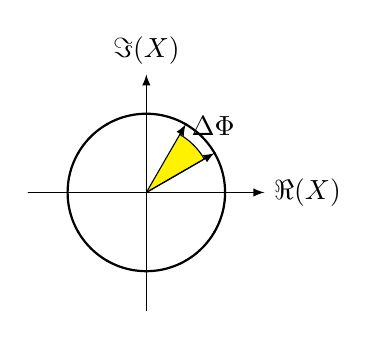
\begin{tikzpicture}[scale=1,cap=round,>=latex]
                    % draw the coordinates
                    \draw[->] (-1.5cm,0cm) -- (1.5cm,0cm) node[right,fill=white] {$\Re(X)$};
                    \draw[->] (0cm,-1.5cm) -- (0cm,1.5cm) node[above,fill=white] {$\Im(X)$};
        
                    \draw[fill=yellow] (0,0) -- (30:.85cm) arc (30:60:.85cm);
                    \draw (45:1.2cm) node {$\Delta\Phi$};
                    \draw[->] (0cm,0cm) -- (0.8660cm,0.5cm);
                    \draw[->] (0cm,0cm) -- (0.5cm,0.8660cm);
        
                    % draw the unit circle
                    \draw[thick] (0cm,0cm) circle(1cm);
            
                    \foreach \x in {0,30,...,360} {
        %	                % dots at each point
                            \filldraw[black] (\x:1cm) circle(0.2pt);
                    }
                \end{tikzpicture}
                \end{tiny}
             \column{0.7\textwidth}
            \begin{itemize}
                \item   frequency and phase change closely related:
                    \begin{itemize}
                        \item<2-> time for full rotation is period length $T$ with \[f = \frac{1}{T}\]
                        \item<3-> time for fractional rotation $\Delta\Phi$ is corresponding fraction of period length \[f = \frac{\Delta\Phi}{\Delta t}\]
                        \item<4-> in other words: 
                        \begin{eqnarray*}
                            \Phi(t) &=& \omega\cdot t\\
                            \Rightarrow \frac{d\Phi(t)}{dt} &=& \omega = 2\pi f
                        \end{eqnarray*}
                    \end{itemize}
            \end{itemize}
            \end{columns}
        \end{frame}
        \begin{frame}{pitch detection resolution}{frequency reassignment: principles}
            frequency domain:
            \begin{itemize}
                \item   instead of using the bin frequency
                    \[ f(k) = k*\frac{f_\mathrm{S}}{\mathcal{K}}\]
                \item   we use the phase of each bin $\Phi(k,n)$
                \item   to compute the frequency from the phase difference of neighboring blocks
                    \begin{equation*}\label{eq:phasediff}
                        \omega_{\mathrm{I}}(k,n)	\propto \Phi(k,n)-\Phi(k,n-1)
                    \end{equation*}
                \item<2->   $\omega_{\mathrm{I}}(k,n)$ is called \textbf{instantaneous frequency} per block per bin
            \end{itemize}
        \end{frame}
        \begin{frame}{pitch detection resolution}{frequency reassignment: scaling factor}
            \begin{itemize}
                \item instantaneous frequency calculation has to take into account
                    \begin{itemize}
                        \item   hop size $\mathcal{H}$
                        \item   sample rate $f_\mathrm{S}$
                    \end{itemize}
                
                    \begin{equation*}
                        \omega_{\mathrm{I}}(k,n) = \frac{\Delta\Phi_{\mathrm{u}}(k,n)}{\mathcal{H}}\cdot f_{\mathrm{S}} 
                    \end{equation*}
                \item<2-> problem: phase ambiguity
                    \begin{equation*}
                        \Phi(k,n) = \Phi(k,n) + j\cdot 2\pi
                    \end{equation*}
                \item<3->[$\Rightarrow$] \textit{phase unwrapping}
            \end{itemize}
        \end{frame}
        \begin{frame}{pitch detection resolution}{frequency reassignment: phase unwrapping}

            \begin{enumerate}
                \item	compute unwrapped phase $\Phi_{\mathrm{u}}(k,n)$ 
                        \begin{itemize}
                            \item	estimate unwrapped bin phase
                                    \begin{footnotesize}
                                    \begin{equation*}\label{eq:phi_est}
                                        \hat{\Phi}(k,n) = \Phi(k,n-1) + \frac{2\pi k}{\mathcal{K}}\mathcal{H} 
                                    \end{equation*}
                                    \end{footnotesize}

                            \item<2->	unwrap phase by shifting current phase to estimate's range
                                    \begin{footnotesize}
                                    \begin{equation*}
                                        \Phi_{\mathrm{u}}(k,n) = \hat{\Phi}(k,n) + \princarg\left[ \Phi(k,n) - \hat{\Phi}(k,n) \right]
                                    \end{equation*}
                                    \end{footnotesize}
                        \end{itemize}

                \item<3->	compute unwrapped phase difference
                        \begin{footnotesize}
                        \begin{eqnarray*}
                            \Delta\Phi_{\mathrm{u}}(k,n)	&=& \Phi_{\mathrm{u}}(k,n) - \Phi(k,n-1)\nonumber\\
                                                \pause
                                                &=& \hat{\Phi}(k,n) + \princarg\left[ \Phi(k,n) - \hat{\Phi}(k,n) \right] - \Phi(k,n-1)\nonumber \\
                                                \pause
                                                &=& \frac{2\pi k}{\mathcal{K}}\mathcal{H} + \princarg\left[ \Phi(k,n) - \Phi(k,n-1) - \frac{2\pi k}{\mathcal{K}}\mathcal{H} \right]\nonumber
                        \end{eqnarray*}
                        \end{footnotesize}
            \end{enumerate}
        
        \end{frame}
        \begin{frame}{pitch detection resolution}{frequency reassignment: problems}
                \begin{itemize}
                    \item   \textbf{overlapping spectral components}
                        \begin{itemize}
                            \item   sinusoidal components often overlap (spectral leakage, several instruments playing the same pitch, ...)
                                \begin{itemize}
                                    \item[$\Rightarrow$] incorrect phase estimate
                                    \bigskip
                                    \item<2-> spectrum should be as sparse as possible, increase STFT length
                                \end{itemize}
                        \end{itemize}
                    \item<3->   \textbf{inaccurate phase unwrapping} 
                        \begin{itemize}
                            \item   unwrapping algorithm is based on assumption of similarity between predicted and measured phase
                            \bigskip
                            \item<2-> decrease hop size
                        \end{itemize}
                \end{itemize}
        \end{frame}
        \begin{frame}{pitch detection resolution}{frequency reassignment: example}
            \figwithmatlab{InstantaneousFreq}
        \end{frame}
        %\begin{frame}{pitch detection resolution}{note on time reassignment, other ways}
        %\end{frame}
        \begin{frame}{pitch detection resolution}{frequency reassignment: matlab exercise}
            \matlabexercise{implementation of the instantaneous frequency computation}
            
            \begin{itemize}
                \item   implement the computation of the instantaneous frequency per block as described int he previous slides
                \item   test for several input sinusoidals with various input frequencies
                    \begin{itemize}
                        \item   detect the local maxima and compare the instantaneous frequency at these bins with both the bin frequency and the original frequency
                    \end{itemize}
            \end{itemize}
        \end{frame}
	%\begin{frame}{frequency detection}{frequency domain resolution: instantaneous frequency 2/2}
		%estimate of instantaneous frequency at bin $k$
		%\begin{footnotesize}
		%\end{footnotesize}
		%
		%\pause
	%\end{frame}
            
   \section[summary]{lecture summary}
        \begin{frame}{summary}{lecture content}
            \begin{enumerate}
                \item       detection resolution is quantized for most pitch detection approaches
                \smallskip
                \item<2->   interpolation approaches can help to virtually improve resolution
                    \begin{itemize}
                        \item   upsampling
                        \item   zero-padding
                        \item   standard interpolation methods
                    \end{itemize}
                \smallskip
                \item<3->   phase-based frequency detection allows an accurate frequency estimate in the spectrum if
                    \begin{itemize}
                        \item   the spectrum is sparse
                        \item   the hop size is small compared to the spectrum
                    \end{itemize}
            \end{enumerate}
        \end{frame}
\end{document}

